\documentclass[12pt]{extarticle}

\usepackage[T1]{fontenc}
\usepackage{polski}
\usepackage[utf8x]{inputenc}
\usepackage[polish]{babel}
\usepackage{url}
\usepackage{afterpage}

\usepackage[margin=1.3in]{geometry}
\usepackage{color}
\usepackage{graphicx}
\usepackage{float}


\begin{document}
\begin{titlepage}
    \begin{center}
        \textsc{\LARGE{Politechnika Śląska}}\\[0.5cm]
        \textsc{\LARGE{Wydział Automatyki, Elektroniki i~Informatyki}}\\[0.5cm]
        \textsc{\LARGE{Kierunek Informatyka}}\\[5.5cm]
        \LARGE{Wypracowanie z przedmiotu Ekonomia}\\[1cm]
        \LARGE{Autor: Aleksander Grzybowski}\\[1cm]
        \LARGE{Gliwice, kwiecień 2017}\\[1cm]
    \end{center}
\end{titlepage}



\section{Rynek, popyt, podaż}

\subsection{Wstęp}

	Dział informatyki zajmujący się algorytmami i strukturami danych zajmuje ważne miejsce w obszarze informatyki teoretycznej. W każdym programie obliczeniowym dobór odpowiednich mechanizmów przetwarzania informacji znacząco wpływa na jego wydajność. Dotyczy to zwłaszcza systemów gromadzenia danych wielkiej skali (tzw. Big Data), które z definicji wymagają przetwarzania w czasie rzeczywistym.

\subsection{Rozwinięcie}

	Kilka typów drzew jest tematem różnych kursów na pierwszym stopniu studiów inżynierskich kierunku Informatyka. Zwykle struktury te są przedstawiane w trakcie wykładów bądź ćwiczeń tablicowych, przy użyciu tradycyjnych slajdów wyświetlanych na rzutniku. Podczas ćwiczeń tablicowych drzewa rysowane są ręcznie, co znacznie utrudnia uchwycenie ich dynamicznej natury, zwłaszcza przy omawianiu różnego rodzaju rotacji. Zdecydowanym ułatwieniem byłoby wykorzystanie programów komputerowych, które umożliwiają wizualizację przebiegu operacji. Narzędzia tego typu uatrakcyjniłyby wykład, a także dałyby studentom możliwość samodzielnego zapoznania się z materiałem w wolnym od zajęć czasie.



\section{Produkcja i koszty w przedsiębiorstwie}


\section{Pieniądz. Polityka monetarna}
\section{Bezrobocie}
\section{Inflacja}


\begin{figure}[H]
\centering
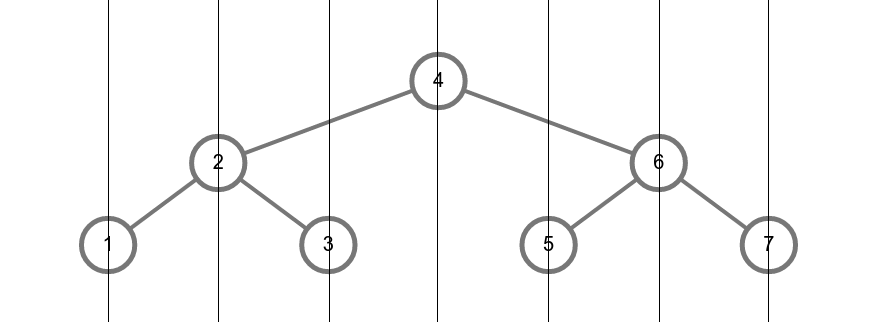
\includegraphics[width=15cm]{sample}
\caption{Jakiś obrazek}
\end{figure}


\begin{enumerate}
	\item Jakaś
	\item Lista
	\item Jakaś
	\item Lista
	\item Jakaś
	\item Lista
\end{enumerate}

\clearpage\mbox{}\clearpage
\end{document}
